\section{Method}\label{sec:method}

DriveCompose converts multi-view image sequences into a compositional Gaussian scene through visual encoding, canonical feature aggregation, latent encoding, joint latent completion, type-specific Gaussian decoding, and scene composition (Fig.~\ref{fig:overview}). Canonical aggregation aligns observations of each component across time; joint completion uses the surrounding scene to infer its missing geometry and appearance.

\subsection{Problem formulation and compositional representation}
\label{sec:representation}

The input is a synchronized image log $\mathbf I_{t,v}$ with timestamps, camera intrinsics, and camera-to-rig calibration. Rig poses are provided or estimated relative to the first frame. Coordinate conventions and image preprocessing are detailed in Appendix D of the supplementary material.

The output is a compositional Gaussian scene

\begin{equation}
\mathcal W=\bigl(\mathcal G_b,C_{\rm sky},V_{\rm sky},
\{\mathcal A_a\},\mathcal B,\xi\bigr),
\label{eq:world}
\end{equation}

where $\mathcal G_b$ is the world-space background, $C_{\rm sky}$ a sky cubemap, $V_{\rm sky}$ its supported directions, $\mathcal A_a$ the canonical asset for identity $a$, $\mathcal B$ the finite spatial support, and $\xi$ the sampling seed. The components are rendered by Gaussian splatting~\cite{kerbl2023gaussians}. Vehicles are represented as rigid assets with fixed local geometry and dimensions. Humans additionally retain a rest skeleton and skinning weights. Scene state controls the placement and articulation of these fixed components.

We model missing content through conditional generation. Let $\mathcal Q$ be the recovered query layout and $C$ its observed evidence. The completion model samples unknown codes $\mathbf z_u$, while the codec $D_\psi$ decodes the assembled codes into scene content:

\begin{equation}
\mathbf z_u\sim p_\theta(\mathbf z_u\mid C,\mathcal Q),
\qquad
\mathcal W=D_\psi(\mathbf z^{\rm obs},\mathbf z_u;\mathcal Q).
\label{eq:generative-reconstruction}
\end{equation}

The query layout assigns each latent code to a spatial location and scene component. Completion fills the unknown codes within this layout, and decoding preserves their component identities and motion bindings.

\subsection{Visual encoding}
\label{sec:visual-encoding}

The Driving Log Encoder extracts patch features from each image and exchanges pooled context across cameras and timestamps~\cite{dosovitskiy2021vit,vaswani2017attention}. Geometry heads predict camera-axis depth, normals, confidence, semantics, and instance assignments. These predictions connect the image features to 3D surfaces and their owning components. Trajectory-level identity slots separate persistent identity, dimensions, and human shape from frame-dependent root poses and joint rotations. Architectural details and state parameterization are given in Appendix D of the supplementary material.

\subsection{Canonical feature aggregation}
\label{sec:queries}

\paragraph{Spatial supports.}

A query stores canonical position $\mathbf q_i$, cell scale $\boldsymbol\delta_i$, type $k_i$, local attention group $g_i$, and reference-world coordinate $\mathbf q_i^w$. Reliable depth samples provide surface anchors. Background anchors are combined with a finite world grid; rigid anchors are aligned by inverse SE(3) transforms and combined with a grid in the local bounding volume. Human queries lie on the canonical template surface. Sky queries are unit directions grouped by cubemap face. These supports provide explicit locations for both observed and missing content.

The layout remains fixed during completion. We obtain $\mathbf q_i^w$ by placing the query in the first input configuration, including skinning for humans. Canonical coordinates identify the content within its component; reference-world coordinates let the generator relate that component to its surroundings.

\paragraph{Motion-aware evidence aggregation.}

For each observation, we place the canonical query at the corresponding actor state:

\begin{equation}
\mathbf p_i(t)=
\begin{cases}
\mathbf q_i,& k_i=\mathrm{background},\\
\operatorname{xyz}(\mathbf T^w_a(t)\bar{\mathbf q}_i),& k_i=\mathrm{rigid},\\
\operatorname{xyz}(\mathbf T^w_h(t)\mathbf A_i(t)\bar{\mathbf q}_i),& k_i=\mathrm{human}.
\end{cases}
\label{eq:query-placement}
\end{equation}

Here $\bar{\mathbf q}_i$ is homogeneous, $\operatorname{xyz}$ extracts Euclidean coordinates, and $\mathbf A_i(t)$ is the weighted skinning transform. Projection gives query depth $z_{i,t,v}$ and samples image features $\boldsymbol\phi_{i,t,v}$, depth $d_{i,t,v}$, and confidence $c_{i,t,v}$. We weight observations by confidence and normalized depth residual $r=(d-z)/(\eta_{\rm abs}+\eta_{\rm rel}d)$. The indicator $a_{i,t,v}$ selects visible, depth-consistent observations of the same instance (Appendix D):

\begin{align}
w_{i,t,v}&=a_{i,t,v}c_{i,t,v}\exp(-r_{i,t,v}^2/2),\\
\mathbf h_i&=\frac{\sum_{t,v}w_{i,t,v}[\boldsymbol\phi_{i,t,v};r_{i,t,v}]}
{\max(\varepsilon,\sum_{t,v}w_{i,t,v})}.
\label{eq:aggregation}
\end{align}

The masks $m_i$, $f_i$, and $u_i$ distinguish observed surfaces, known free space, and unknown content, with $m_i+f_i+u_i=1$. Confidence is the maximum over valid observations; free space is inferred from reliable depth rays. Sky features are aggregated by viewing direction using camera rotation and sky semantics. Appendix D gives the visibility and free-space criteria.

\subsection{Latent representation encoding}
\label{sec:codec}

Type-specific encoders compress the aggregated feature and its spatial support, $[\mathbf h_i;\mathbf q_i;\boldsymbol\delta_i]$, into a latent code $\mathbf z_i\in\mathbb R^D$. The shared latent dimension lets the completion model exchange information across background, rigid, and human representations. Each query keeps its type, ownership, and coordinate frame even though all codes have the same dimension. Visibility masks and confidence are supplied separately to the completion model. Partial and complete observations therefore use the same intrinsic encoding map. Before conditioning, unobserved codes are set to zero; the observed subset is denoted $\mathbf z^{\rm obs}$.

\subsection{Joint latent-space completion}
\label{sec:completion}

\begin{figure*}[t]
  \centering
  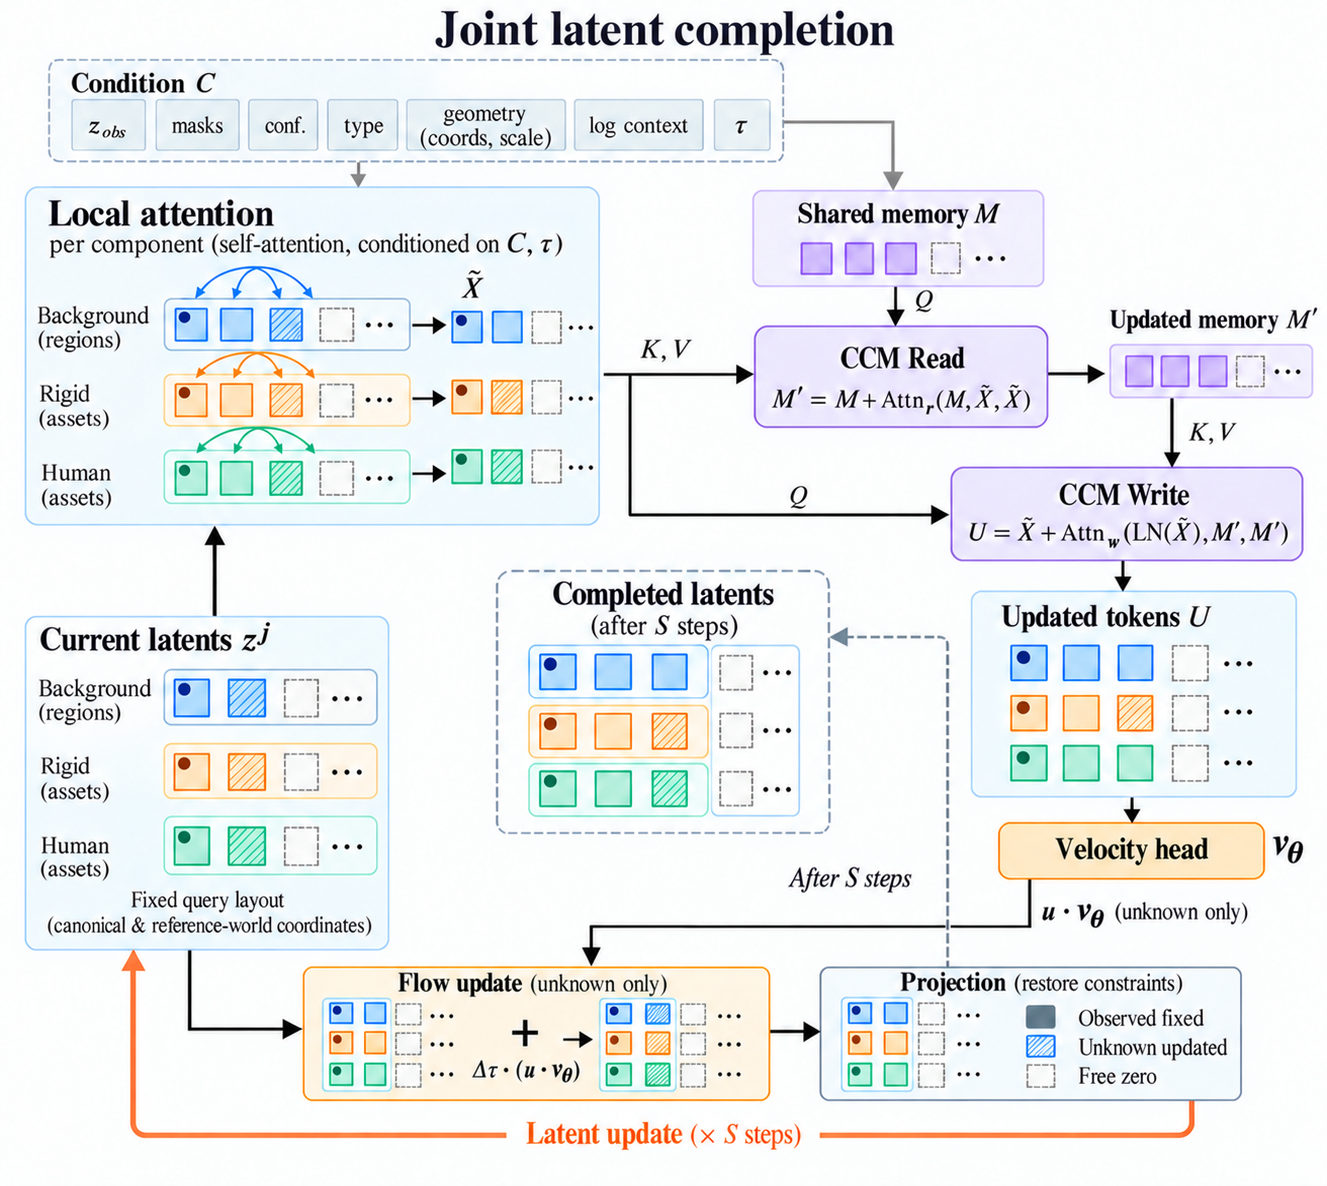
\includegraphics[width=0.86\textwidth]{fig/drivecompose-joint-completion.png}
  \caption{\textbf{Joint latent completion.} Group-local attention updates component features; CCM reads them into shared memory and writes context back to every component. The velocity head drives unknown-code updates. Projection restores observed codes and clears free-space codes after each step, with the query layout fixed. Completed codes are taken after the final projection.}
  \label{fig:joint-completion}
\end{figure*}

\paragraph{Generative completion module.}

Our generative completion module (GCM) combines a scene-conditioned flow transformer with constrained sampling (Fig.~\ref{fig:joint-completion}). We parameterize its completion velocity with a DiT-style transformer~\cite{peebles2023dit} trained by flow matching~\cite{lipman2022flowmatching}. Its input combines current and observed codes, masks, confidence, type, both coordinate descriptions, cell scales, and pooled log features. Background groups follow spatial neighborhoods, each asset forms a local group, and sky directions are grouped by cubemap face. Local self-attention processes these groups separately. A cross-component memory (CCM) module then exchanges context through shared memory:

\begin{align}
\mathbf M'&=\mathbf M+\operatorname{Attn}_{r}
(\mathbf M,\widetilde{\mathbf X},\widetilde{\mathbf X}),\\
\mathbf U&=\widetilde{\mathbf X}+\operatorname{Attn}_{w}
(\operatorname{LN}(\widetilde{\mathbf X}),\mathbf M',\mathbf M').
\label{eq:memory-exchange}
\end{align}

Here $\widetilde{\mathbf X}$ concatenates locally updated tokens, and attention arguments are queries, keys, and values. A residual feed-forward update follows $\mathbf U$. Flow-time modulation enters the local normalization; learned tokens and log summaries initialize memory. This structure keeps each support's local organization while allowing a rigid or human query to use information from the surrounding scene.

\paragraph{Flow training and constrained sampling.}

Let $\mathbf z_1$ be a complete target on the same query layout and $\boldsymbol\epsilon\sim\mathcal N(0,\mathbf I)$ be Gaussian noise. We interpolate only the unknown content at flow time $\tau\in[0,1]$:

\begin{equation}
\mathbf z_\tau=m\odot\mathbf z^{\rm obs}
+u\odot[(1-\tau)\boldsymbol\epsilon+\tau\mathbf z_1].
\label{eq:flow-path}
\end{equation}

Observed codes remain fixed and free-space codes remain zero. The target velocity for unknown queries is $\mathbf z_1-\boldsymbol\epsilon$. With an optional loss selector $s_i$, the objective is

\begin{equation}
\mathcal L_{\rm flow}=
\frac{\sum_i u_i s_i\|\mathbf v_\theta(\mathbf z_\tau,\tau,C)_i
-(\mathbf z_{1,i}-\boldsymbol\epsilon_i)\|_2^2}
{D\max(1,\sum_i u_i s_i)}.
\label{eq:flow-loss}
\end{equation}

Complete scene or asset examples supply $\mathbf z_1$ at the unknown queries, while $s_i$ selects their contribution to the training loss (Sec.~\ref{sec:training}).

At inference, we initialize unknown codes with noise and take $S$ Euler steps with $\Delta\tau=1/S$:

\begin{equation}
\mathbf z^{j+1}=\Pi_{m,f}\!\left[
\mathbf z^j+\Delta\tau\,u\odot
\mathbf v_\theta(\mathbf z^j,j/S,C)\right].
\label{eq:sampling}
\end{equation}

The projection $\Pi_{m,f}$ restores observed codes and clears free-space codes after every step. The seed fixes one sampled completion. Sampling precedes decoding, and the resulting scene is reused when the camera or actor states change.

\subsection{Type-specific Gaussian decoding}
\label{sec:decoding}

Background, rigid, and human Gaussian decoders independently map each query to $K$ child Gaussians confined to its support cell. Human children inherit the query's skinning weights; rigid children share their asset's rigid transform. Opacity is multiplied by $1-f_i$, so free queries cannot produce visible Gaussians. A separate sky head predicts cubemap colors within the observation-supported domain $V_{\rm sky}$. Gaussian and appearance parameterizations are detailed in Appendix E of the supplementary material.

Each query is decoded independently. Freezing the codec and retaining observed codes therefore preserves the Gaussian parameters of observed surfaces.

\subsection{Scene composition}
\label{sec:composition}

\paragraph{State-driven rendering.}

At time step $k$, state $s_k$ specifies the ego pose, active assets, rigid transforms, and human root and joint poses. Rigid poses transform canonical Gaussian centers and covariances rigidly. Human joint poses deform them through the stored skinning weights, so completed surfaces move with the corresponding body parts. Appendix C gives the transformations. The renderer composites the background, active assets, and valid sky:

\begin{equation}
o_k=\mathcal R(\operatorname{Compose}(\mathcal W,s_k),\mathcal C_k).
\label{eq:simulation}
\end{equation}

Changing the camera selects a new view of the composed scene; changing an actor state moves its completed canonical asset. The background and canonical content remain fixed across these operations, allowing the same reconstruction to be reused along different trajectories.

\subsection{Training procedure}
\label{sec:training}

We train visual recovery, the latent codec, and the completion model in sequence, then adapt completion through rendered observations (Table~\ref{tab:training}). Freezing the codec during completion training keeps its target latent space fixed.

\begin{table}[t]
\centering
\small
\caption{Training schedule. R: recovery; C: codec; G: GCM. T: trained; F: frozen; --: unused.}
\label{tab:training}
\begin{tabular}{@{}lccc p{0.43\linewidth}@{}}
\toprule
Stage & R & C & G & Supervision \\
\midrule
Recovery & T & -- & -- & Geometry, semantics, identity, states \\
Codec & F & T & -- & Partial / complete observations \\
Prior & F & F & T & Complete targets \\
Adaptation & F & F & T & Real-log rendering and scene constraints \\
\bottomrule
\end{tabular}
\end{table}

For codec fitting, partial input and more complete observations share the same query positions, types, order, and ownership. With recovery and the entire codec frozen, complete scene or asset examples provide a valid target for every unknown query to train the GCM with Eq.~\ref{eq:flow-loss}. Real-log adaptation differentiates through flow integration, decoding, and rendering to update only the GCM. Complete-target samples can be interleaved to retain the prior, with each loss applied only to samples carrying its required targets. Observed anchors are enforced by frozen decoding and hard code restoration. Detailed supervision, losses, and conditioning perturbations are provided in Appendix B of the supplementary material.
